\subsection{采访刘艳老师}
\subsubsection{刘艳老师介绍}
刘艳,女,硕士,讲师,心理中心专职咨询师。中国心理学会临床心理学注册工作委员会注册心理师,国家二级心理咨询师,
国际聚焦取向咨询师(FOT)。16年心理学专业熏陶,13年分析心理学受训,10年人本主义聚焦取向心理学受训。从事心理咨询工作10余年,
个体咨询5000小时以上,团体咨询1000小时以上。
个案类型集中在大学生、儿童青少年与成年女性。
工作风格乃以分析心理学为主的动力学取向,整合沙盘游戏等表达性疗法与聚焦疗法。
\subsubsection{采访节选}
问:您对``容貌焦虑''有哪些了解?

答:``容貌焦虑''并非明确的心理或精神障碍诊断概念,只是社会上的流行说法。它涵盖了人们对外在形象是否符合某种标准的担忧,可实际上根本没有这样的标准。在真实生活中,相处久了,大家不会仅凭容貌定义一个人。但社会上存在一种认知,觉得漂亮很重要,似乎要达到某个不知从何而来的标准。

我遇到过一些情况,有人觉得必须整容,否则大学都读不下去,甚至日子都过不下去。这种``容貌焦虑''是一种外在表现,是担心容貌不够好而失去某些东西。
社会心理学对此有研究,比如韩国整容业发达,是因为在韩国有一种社会认知:长得漂亮意味着拥有其他美好品质,打扮好、长得好的人可能更精明或有更多权力,在事业等方面表现更好,这就像晕轮效应,因外貌给人加上光环。这种社会认知与国家或集体的经济发展水平、社会形态、历史发展阶段都有关系。

在我国,这种现象在21世纪后变得比较夸张,担心容貌影响自身发展只是表象。从我的接触来看,有``容貌焦虑''的人,可能自尊水平很低,无法确定自己不管化不化妆都能被他人接受,所以必须呈现出完美的一面才放心。他们的安全感也可能较差,或许还曾因他人以审视的目光对待自己而受伤,比如社会推崇两米的身高为理想型,很多人达不到,这种社会潮流很容易形成,也很容易用一种社会认知去打击一群人。但每个人的承受能力不同,有的人由于成长经历,没有强大的内心,真的难以承受。

问:如何克服``容貌焦虑''呢?

答:比较简单的方法就像我们刚才提到的,要塑造自己的内核。真正去发现自己的多个方面,要知道自己拥有很多资源。即便没有刻意打扮自己,我们依然可以对自己有良好的感觉。比如说,有一次同学们为我鼓掌,不是因为我化了妆,我甚至都不清楚自己做了什么,但同学们就是喜欢和我在一起。如果这样的经历越来越多,我们就越不需要依靠那些外在的堆砌了。
其实每个人都应该多花些心思在自己身上。现在,我们把太多精力放在关注别人创造的内容上了,比如短视频,却太少进行自我反思,将注意力回归自身。我们已经太久忽略了和自己内心的联系,甚至把这种自我关注看作是无用的,将其价值贬低、功利化。似乎什么都可以被功利化,但这样我们却失去了一些本真的东西。

当我们深入钻研这个话题到一定程度时,其实可以倡导一种新的社会文化。就像之前提到的那种单一的审美标准,比如``两米才是美''这种观念,我们可以推翻它,构建一个多元文化的世界,鼓励每个人更多地关注自身。如果我们去倡导这样的理念,社会会不会因此发生一些改变呢?会不会让那些深受容貌焦虑困扰的人得到解脱呢?我们可以试着把问题反过来思考。

就像我们之前在做女性相关宣传的时候,以一个知名女性内衣品牌为例,在它的广告里,不同高矮、胖瘦、民族、肤色的女性穿上内衣都展现出自信。如果我们多传播这样的信息,有没有可能给社会带来一些积极的改变呢?所以,除了个人要塑造稳定的内核,我们还需要创造不一样的文化,这样才能让更多人摆脱困扰,让大家不再为此担忧。

\subsubsection{总结}
``容貌焦虑'' 并非专业的心理或精神障碍诊断概念,而是社会上流行的说法,其根源在于大众追捧却又虚幻无依据的 ``美貌标准'',人们会担忧自身外在形象不符合这种莫须有的标准,进而产生焦虑。

``容貌焦虑''的起因是多方面的。从个体心理角度看,人类天生具有被认可、被接纳的需求,而在现代社会中,容貌往往被视为获取认可的重要途径之一。尤其是对于那些自尊水平较低、安全感不足的个体,他们更依赖外在的容貌评价来构建自我价值感。

其实,``容貌焦虑''也不过是纸老虎,战胜它很容易。首先要重塑强大的 ``内核'',通过挖掘自身多元价值,珍视那些与容貌无关的被认可时刻,将注意力从外界纷扰回归到内心本真,减少对外在容貌的过度依赖,增强自我认同感。同时,社会需要摒弃单一审美标准这种 ``毒瘤'',构建多元包容的文化,倡导多元美的信息,打破刻板审美禁锢,从整体文化氛围上帮助人们摆脱容貌焦虑的困扰。

\subsection{采访同学}
问:你认为你存在容貌焦虑吗?你是如何判断的?

答:存在。我觉得这是基于一定的水准,内心有着想往更加向善向好的容貌方向发展的渴望,同时也夹杂着一种焦虑感和攀比心理吧。

问:你认为你的这种审美认识是如何产生的呢?

答:可能是源于平时看的一些篮球赛事片段,还有对电影明星形象的印象吧。

采访同学,我们知道了一些同学容貌焦虑的直接诱因,和形成的心理过程。
\begin{figure}[H]
    \centering
    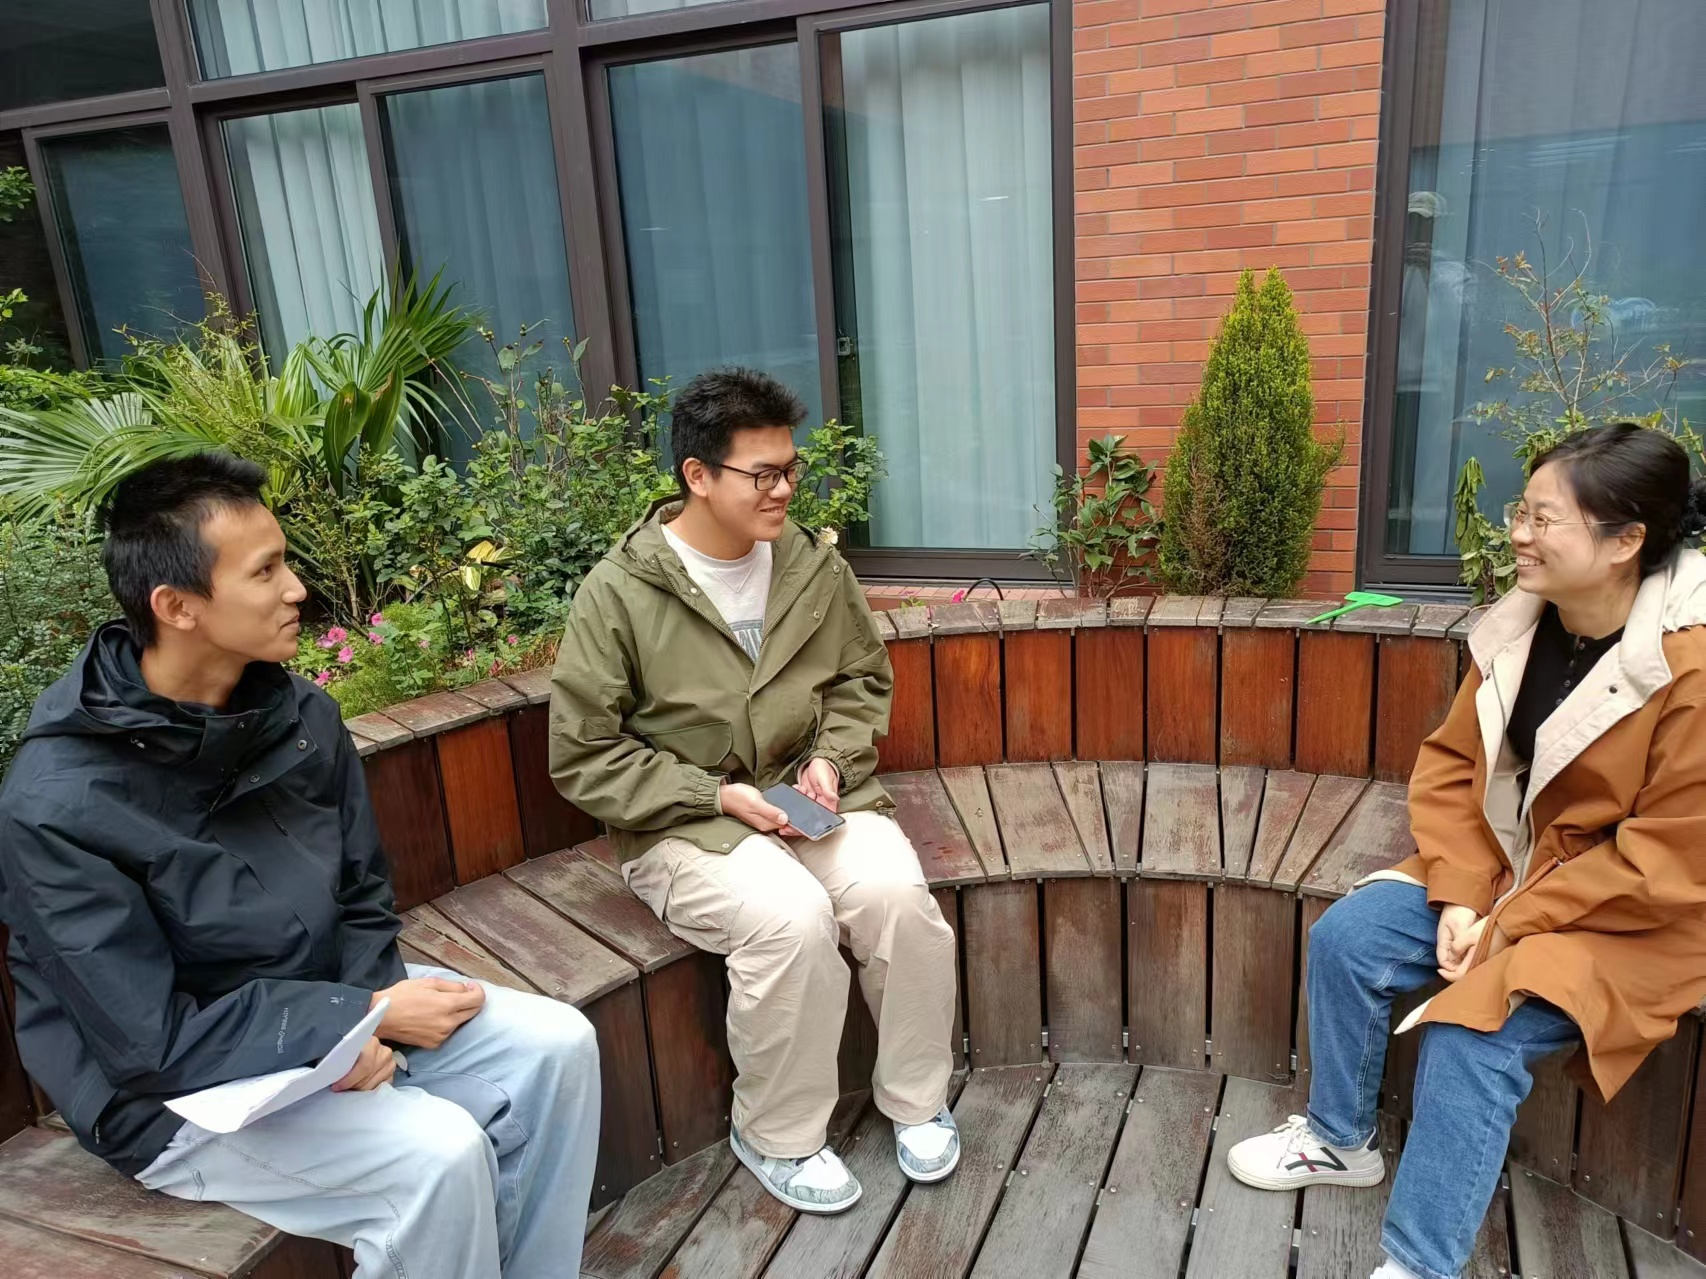
\includegraphics[width=0.7\textwidth]{./assets/采访.jpg}
    \caption{采访图片}
\end{figure}